\cotefile{36}
\scanpage{38}\mspage{- 98 -}\hfill n\textsuperscript{o} 316
% archive sheet number: 37

un automorphisme de $E$.

Si en outre $E$ est une algèbre (non nécessairement associative), et si $u$ est une dérivation (nilpotente) de $E$, alors $e^u$ est un automorphisme de \uline{l'algèbre} $E$. En effet, si $x,y\in E$, on a
\[
u^p(xy)=\sum\nolimits_{r+s=p}\binom{p}{r}\,u^r(x)\,u^s(y)
\]
pour tout entier $p\geqslant 0$ (formule de Leibniz). Il en résulte que :
\[
\begin{aligned}
e^u(xy)&=\sum\nolimits_{p\geqslant 0}\frac{1}{p!}\,u^p(xy)
=\sum\nolimits_{p\geqslant 0}\sum\nolimits_{r+s=p}\frac{u^r(x)}{r!}\,\frac{u^s(y)}{s!}\\
&=\sum\nolimits_{r,s=0}^{\infty}\frac{u^r(x)}{r!}\,\frac{u^s(y)}{s!}
=e^u(x)\,e^u(y)
\end{aligned}
\]
d'où notre assertion.

Soit maintenant $\unsure{\mathbb{g}|g}$ une algèbre de Lie. Si $x$ appartient au radical nilpotent de $\mathbb{g}$, la dérivation $\mathrm{ad}_{\mathbb{g}}\,x$ de $\mathbb{g}$ est nilpotente. On peut donc poser la définition suivante :

\uline{Définition} 5 - \uline{On appelle automorphisme spécial de} $\mathbb{g}$ \uline{un automorphisme de} $\mathbb{g}$ \uline{de la forme} $e^{\mathrm{ad}\,x}$, \uline{où} $x$ \uline{est dans le radical nilpotent de} $\mathbb{g}$.

Il est clair qu'un automorphisme spécial laisse stable tout idéal de $\mathbb{g}$.

\uline{Définition} 6 - \uline{Soient} $\mathbb{g}$ \uline{une algèbre de Lie}, $\unsure{\mathbb{r}|r}$ \uline{son radical}. \uline{On appelle sous-algèbre de Levi de} $\mathbb{g}$ \uline{toute sous-algèbre supplémentaire de} $\mathbb{r}$ \uline{dans} $\mathbb{g}$.

Une sous-algèbre de Levi est isomorphe à $\mathbb{g}/\mathbb{r}$, donc semi-simple. Comme une sous-algèbre semi-simple n'a que $0$ en commun avec $\mathbb{r}$, toute sous-algèbre semi-simple $\unsure{\mathbb{h}|h}$ telle que $\mathbb{g}=\mathbb{r}+\mathbb{h}$ est une sous-algèbre de Levi ; par conséquent, l'image d'une sous-algèbre de Levi par un homomorphisme surjectif est une sous-algèbre de Levi.
\scanpage{39}
% archive sheet number: 38
$X$ propre et simple sur $k$ [\unsure{généralisons|généraliser|généralisations} à une base quelconque]

$A$ V.A. sur $k$

$H^1(X,A)=\underset{n}{\underrightarrow{\lim}}\,{}_{n}H^1(X,A)\ \deleted{\unsure{=|.|;}}$ \enspace d'autre part, on a une suite exacte
\[
0\longrightarrow\mathrm{Hom}(X,A)_{n}\longrightarrow\deleted{{}_{\unsure{n}}}H^1(X,{}_{n}A)\longrightarrow{}_{n}H^1(X,A)\longrightarrow 0
\]
qui s'écrit aussi
\[
0\longrightarrow\mathrm{Hom}(\mathrm{Alb}_{X},A)_{n}\longrightarrow\mathrm{Hom}(D({}_{n}A),\mathrm{Pic}_{X})\longrightarrow{}_{n}H^1(X,A)\longrightarrow 0
\]
\unsure{ou enfin|on a enfin}, notant que
\[
\begin{aligned}
\mathrm{Hom}(\mathrm{Alb}_{X},A)&\simeq\mathrm{Hom}(A',(\mathrm{Alb}_{X})')=\mathrm{Hom}(A',\mathrm{Pic}^{0}_{X})\\
D({}_{n}A)&\simeq{}_{n}A'
\end{aligned}
\]
une suite exacte
\makeatletter\tagsleft@true\makeatother
\[
0\longrightarrow\mathrm{Hom}(A',\mathrm{Pic}^{\unsure{0}}_{X})_{n}\longrightarrow\mathrm{Hom}({}_{n}A',\mathrm{Pic}_{X})\longrightarrow{}_{n}H^1(X,A)\longrightarrow0
\tag*{(*)}
\]
et passant à la limite \inserted{\unsure{inductive}} sur $n$ :
\[
\boxed{0\longrightarrow\mathrm{Hom}(A',\underline{\mathrm{Pic}}^{0}_{X})\otimes_{\mathbb Z}\mathbb Q\longrightarrow\mathrm{Hom}(T_{\cdot}(A'),\underline{\mathrm{Pic}}_{X})\longrightarrow H^1(X,A)\longrightarrow0}
\]
Or la suite exacte $(*)$ se compare à la suite exacte déduite de $0\mathbin{\unsure{-|\to}}{}_{n}A'\mathbin{\unsure{-|\to}} A'\longrightarrow A'\longrightarrow0$ en appliquant $\deleted{\unsure{\mathrm{Ext}^{1}|\mathrm{Ext}}}\underline{\mathrm{Hom}}(-,\mathrm{Pic}_{X})$, on trouve
\[
0\longrightarrow\mathrm{Hom}(A',\underline{\mathrm{Pic}}_{X})_{n}\longrightarrow\mathrm{Hom}({}_{n}A',\underline{\mathrm{Pic}}_{X})\longrightarrow{}_{n}\mathrm{Ext}^{1}(A',\underline{\mathrm{Pic}}^{\unsure{2|0}}_{X})\longrightarrow0
\tag*{(**)}
\]
qui donne à la limite
\[
\boxed{0\mathbin{\unsure{-|\to}}\mathrm{Hom}(A',\mathrm{Pic}_{X})\otimes_{\mathbb Z}\mathbb Q\longrightarrow\mathrm{Hom}(T_{\cdot}(A'),\mathrm{Pic}_{X})\longrightarrow\mathrm{Ext}^{1}(A',\underline{\mathrm{Pic}}_{X})_{\unsure{n|\mathrm{t}}}\ \unsure{\supset|0}}
\]
\makeatletter\tagsleft@false\makeatother
\scanpage{40}
% archive sheet number: 39
On en conclut un isom canonique
\[
\boxed{H^1(X,A)\mathrel{\overset{\sim}{\longleftarrow}}\mathrm{Ext}^{1}(A',\underline{\mathrm{Pic}}_{X})}
\]
\margin{Cet isomorphisme reste-t-il valable pour $X$ singulier ??? Il est possible qu'on ait besoin de $H^i(X,G_m)=0$ pour $i\geqslant2$, qui \unsure{est douteux si|est douteux en} $X$ non rég ??}
($A$, variété abélienne), qu'on comparera à la formule de dualité
\[
\boxed{H^1(X,G)\simeq\mathrm{Hom}(D(G),\underline{\mathrm{Pic}}_{X})}
\]
pour $G$ commutatif affine.

Remarque, On a des hom canoniques
\diagram{\begin{tikzcd}[ampersand replacement=\&]
\mathrm{Ext}^{1}(\underline{\mathrm{Alb}}_{X},A) \arrow[r] \arrow[d,"\wr"] \& H^1(X,A)\\
\mathrm{Ext}^{1}(A',\underline{\mathrm{Alb}}_{X}{}') \arrow[d,"\unsure{\wr|\sim}"] \& \\
\mathrm{Ext}^{1}(A',\underline{\mathrm{Pic}}^{\tau}) \&
\end{tikzcd}}
dont on montre que c'est des \uline{isomorphismes dans}, qui définissent sur les sous groupes en question l'isomorphisme envisagé plus haut.
\scanpage{41}
% archive sheet number: 40
\[
\boxed{\underline{\mathscr H}^{1}(X/S;\underline{\mathrm{Hom}}_{S\text{-}\mathrm{gr}}(\gamma,G))\mathrel{\overset{\sim}{\longrightarrow}}\underline{\mathrm{Hom}}_{S\text{-}\mathrm{gr}}(\gamma,\underline{\mathscr H}^{1}(X/S;G))}
\]
\diagram{\begin{tikzcd}[ampersand replacement=\&]
X\arrow[d]\\S
\end{tikzcd}}
isom de foncteurs, \deleted{\unsure{pour}} quand tout est \uline{affine} sur $S$ (?)
\[
\boxed{\underline{\mathscr H}^{1}(X/S;\underline{\mathrm{Ext}}^{1}_{S\text{-}\mathrm{gr}}(\gamma,G))\simeq\underline{\mathrm{Ext}}^{1}_{S\text{-}\mathrm{gr}}(\gamma,\mathscr H^{1}(X/S;G))}
\]
Sous quelles conditions ???

\diagram{\begin{tikzcd}[ampersand replacement=\&]
\& \unsure{P|\rho}_{X}\&\\
X\arrow[d,dash] \& \deleted{\gamma_{X}}\unsure{X_{\gamma}|\gamma_X} \& \deleted{\unsure{\gamma_{X}\times\gamma_{X}|X_{\gamma\times\gamma}}}\unsure{X_{\gamma\times\gamma}|\gamma_{X}\times\gamma_{X}}\\
S\&\gamma\&\gamma\times\gamma
\end{tikzcd}}
\[
\mathscr H^1(X/S,\underline{\mathrm{Hom}}_{S\text{-}\mathrm{gr}}(\gamma,G))\longrightarrow\mathrm{Hom}(\gamma,\mathscr H^1(X/S,G))
\]
\[
\mathscr H^1(X,\mathrm{Hom}(A;B))\simeq
\]
$\deleted{\unsure{E(X/S,|F(X/S,|E(A,B,}}$
\diagram{\fbox{\begin{tikzcd}[ampersand replacement=\&]
H^1(X/S;\underline{\mathrm{Hom}}_{S\text{-}\mathrm{gr}}(\gamma,G))\arrow[d]\\
\underline{\mathrm{Hom}}_{S\text{-}\mathrm{gr}}(\gamma,H^1(X/S;G))
\end{tikzcd}}}
\scanpage{42}
% archive sheet number: 41
\deleted{\diagram{\begin{tikzcd}[ampersand replacement=\&]
f^{-1}(U)\arrow[r,hook,"i"]\arrow[d,"f"]\&X\arrow[d,"f"]\\
U\arrow[r,"j"']\arrow[ur,"g"']\arrow[u,bend right=19,decorate,decoration={snake,amplitude=.4mm,segment length=2mm},"\deleted{\unsure{g}}"]\&Y
\end{tikzcd}}
\[
\begin{aligned}gf&=i\\fg&=j\end{aligned}
\]
$f$ morphisme birationnel \inserted{propre} de préschémas intègres $X,Y$

$U$ ouvert de $Y$ sur lequel $f^{-1}$ est défini [Si $Y$ est régulier en codim $1$, alors $U$ est le \unsure{complémentaire} d'\unsure{un|une} ens de codim $\geqslant2$], \deleted{\unsure{i.e. aussi les pts|i.e. ens des pts}} \unsure{i.e., aussi les pts|i.e., ensemble pts} ayant un voisinage $V$ tel que $f$ induise un isom $f^{-1}(U)\longrightarrow V$.

Soit $\xi\in\mathrm{Pic}(X)$ défini par un \inserted{\uline{cycle}} \uline{divisoriel} $D$ (\unsure{$X$ ouvert|$X$ connex|$X$ normal}), considérons \deleted{\unsure{un}} \deleted{le morphisme} $g^{-1}(\xi)\in\mathrm{Pic}(U)$, il correspond à un cycle divisoriel}
\scanpage{43}
% archive sheet number: 42
\diagram{\begin{tikzcd}[ampersand replacement=\&]
\mathscr H^1(X;A)\arrow[d,dash]\&\mathrm{Ext}^1(A,\mathrm{Pic})\\
\text{pt singulier}\&
\end{tikzcd}}
\[
\boxed{\mathscr H^1(X,G)\simeq\mathrm{Hom}(D(G),\underline{\mathrm{Pic}}_{X})}
\]
\figure{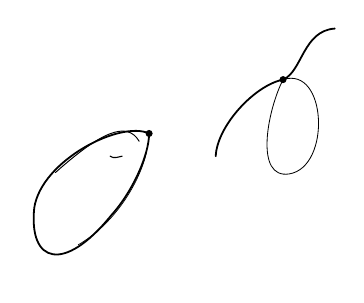
\begin{tikzpicture}[x=.009cm,y=-.009cm,line cap=round,line join=round]
\draw[line width=.65pt] (165,152) .. controls (125,133) and (13,190) .. (3,257) .. controls (-5,335) and (45,350) .. (112,267) .. controls (141,235) and (165,183) .. (165,152);
\draw[line width=.35pt] (33,207) .. controls (98,149) and (134,134) .. (151,163);
\draw[line width=.25pt] (65,309) .. controls (116,280) and (151,222) .. (161,180);
\draw (110,184) .. controls (115,188) and (122,185) .. (127,184);
\fill (165,152) circle (5);
\draw[line width=.65pt] (259,184) .. controls (261,141) and (314,84) .. (354,76) .. controls (381,65) and (382,7) .. (427,4);
\draw[line width=.3pt] (354,76) .. controls (332,119) and (313,217) .. (363,209) .. controls (422,199) and (416,56) .. (354,76);
\fill (354,76) circle (5);
\end{tikzpicture}}
\[
\mathscr H^{i}(X,D(G))\simeq\mathrm{Ext}^{i}(G,\underline{\mathrm{Pic}}_{X})
\]
\[
\mathrm{Ext}^{i}_{X}(f^{!}(G),G_{m\unsure{,|{}}})\simeq\mathrm{Ext}^{i}_{Y}(G,f_{!}(G_{m}))
\]
\diagram{\begin{tikzcd}[ampersand replacement=\&]
X\arrow[d,"f"']\\Y
\end{tikzcd}}
\[
\boxed{\underline{\mathrm{Ext}}^{i}_{X}(f^{*}(G_{\cdot}),H^{\cdot})\simeq\underline{\mathrm{Ext}}^{i}_{Y}(G_{\cdot},f_{!}(H^{\cdot}))}
\]
\[
H=G_m
\]
\[
\underline{\mathrm{Ext}}^{i}_{X}(f^{*}(G),G_{m})\simeq\underline{\mathrm{Ext}}^{i}_{Y}(G,\overset{\text{\unsure{les supérieurs}}}{\tikz[baseline=(p.base)]\node[draw,ellipse,inner sep=2pt](p){$\underline{\mathrm{Pic}}^{\bullet}_{X/Y}$};})
\]
\[
\begin{aligned}
&\deleted{\unsure{f|R}}&&&&\Vert\\
&\deleted{\unsure{H^p(X,|H^i(X,}}&&\Vert
\end{aligned}
\]
\[
\boxed{G\text{ \uline{affine}, alors}\quad H^{i}(X,D(G))\Longleftarrow\deleted{\unsure{\mathscr H}}\mathrm{Ext}^{p}(G,\mathrm{Pic}^{(q)}_{X/Y})}
\]
\[
\begin{aligned}
\unsure{i|j}=0\qquad&H^0(X,D(G))=\deleted{\unsure{\mathrm{Hom}}}D(G)\\
i=1\qquad&H^1(X,D(G))=\deleted{\unsure{\mathrm{Ex}|\mathrm{Ext}}}\mathrm{Hom}(G,\mathrm{Pic}^{(1)})\\
i=2\qquad&\underline{H^2(X,D(\unsure{e|G}))\mathrel{\#}\mathrm{Ext}^1(G,\mathrm{Pic}^{(1)}_{X/Y})+\mathrm{Hom}(G,\underline{\mathrm{Pic}}^{\unsure{(2)}}_{X})}\\[-2pt]
&\hspace{4em}\text{!}
\end{aligned}
\]
$G$ abélien \quad Alors \quad \unsure{chg|sg}
\[
H^{i-1}(X,G')\Longleftarrow\mathrm{Ext}^{p}_{\unsure{\mathrm{gr}|Y}}(G,\mathrm{Pic}^{q}_{X/Y})
\]
\[
\begin{aligned}
i=0\qquad&0=0\\
i=1\qquad&H^{0}(X,G')=
\end{aligned}
\]
\scanpage{44}
% archive sheet number: 43
\uline{Foncteurs adjoints}

\uline{Definition 1} Soient $X,Y\in(\mathrm{Cat})$, $f:X\to Y$ et $g:Y\unsure{\text{---}|\to}X$, on dit que $(f,g)$ est un couple de foncteurs adjoints, ou que $g$ est adjoint de $f$, ou que $f$ est coadjoint de $g$, s'il existe un

\figure{\begin{tikzpicture}[x=.012cm,y=.012cm]
\draw (0,0)--(230,-2)--(48,-20)--(106,-57)--(99,13)--(104,-107)--(145,15)--(146,-84);
\draw (264,1)--(825,-23);
\draw (252,-15)--(-188,-610)--(-670,-582);
\draw (-188,-610)--(-666,-628);
\end{tikzpicture}}

\[
\begin{aligned}
&\mathscr H^{\unsure{1|{}}}(X,\underline{\operatorname{Hom}}(\gamma,G))\simeq\\
&\mathscr H^1(X,\underline{\operatorname{Ext}}^1(\gamma,G))\\
&\operatorname{Ext}^1(\gamma,
\end{aligned}
\]
\[
\begin{aligned}
&X\unsure{\text{---}|\to}\underline{\operatorname{Hom}}_{S\text{-gr}}(\gamma,G)\\
&X\times\gamma\longrightarrow G
\end{aligned}
\]
\diagram{\begin{tikzcd}[ampersand replacement=\&]
\deleted{\unsure{\gamma|g}}\,\gamma \arrow[r] \arrow[dr,dash] \& \underline{\operatorname{Hom}}_{S}(X,G)\\
S \& \overset{\unsure{P_2|P_r}}{\unsure{C|G}}
\end{tikzcd}}
\[
\operatorname{Hom}(\gamma,
\]
\[
\begin{aligned}
&\prod_{X/S}^{0}\gamma_X\\
&\quad\Vert\\
&\underline{\operatorname{Hom}}_S(X,\gamma)\unsure{-|=|\doteq}\gamma
\end{aligned}
\]
\[
e\to\gamma\to\underline{\operatorname{Hom}}_S((X,\gamma)\longrightarrow
\operatorname{Hom}(X,\unsure{a|0}\mathbin{;}\gamma)\to0
\]
\scanpage{45}
% archive sheet number: 44
D'après la théorie d'Artin-Schreier-Witt, on a
\[
H^1(A,\mathbb Z/p)\simeq H^1(A,\underline O_A)_{\deleted{\unsure{p|s}}}^{(p)}
\qquad \text{éléments de } H^1(A,\underline O_A)\text{ tels que } Fx=x
\]
\[
H^1(A,\mathbb Z/p^{\unsure{n|m}})\simeq
H^1(\deleted{\unsure{O|A}}A,\underline O_A(W_n))^{(p)}
\qquad \text{--- }H^1(A,\underline O_A(W_n))\text{ tels que }Fx=x
\]
\[
\boxed{\operatorname{Hom}(\pi_1^p(A),\mathbb Z_p)\simeq H^1(A,\deleted{\unsure{\mathbb Q_p|\underline O_p}}\mathbb Z_p)
\simeq H^1(A,W)_{\deleted{\unsure{s|p}}}^{(p)}}
\]
\deleted{\unsure{idem|idée}} \inserted{\unsure{dont|d'où}} \deleted{\unsure{on}} on déduit un \deleted{accouplement} isomorphisme
\[
\boxed{\deleted{\pi_1^p(A)\times H^1(A,W)_s\longrightarrow\mathbb Z_p}}
\]
qui est une dualité \deleted{\unsure{de|(?)}} de $\mathbb Z_p$-modules libres de type fini
\[
\boxed{\deleted{\operatorname{Hom}_{\unsure{\mathrm{cont}|\mathrm{ant}}}(\pi_1^p(A),\Lambda)\simeq H^1(A,W)_s}}
\]

D'autre part, utilisant encore le fait que tout revêtement de $A$ est une variété abélienne, on trouve aussi
\[
\boxed{\pi_1^p(A)\simeq T_p(A)}
\]
d'où en les \unsure{comparant|composant}
\[
\boxed{T_p(A)\times H^1(A,W)^{(p)}\longrightarrow\mathbb Z_p}
\]
qui est une dualité de $\mathbb Z_p$-modules libres de type fini.

\deleted{qu'on peut aussi écrire} \unsure{dont|donc|d'où|dans} on déduit
\[
\boxed{\operatorname{Hom}_{\unsure{\mathrm{cont}|\mathrm{ant}}}(T_p(A),\deleted{\unsure{\mathbb Z|\Lambda}}W_{\infty}(k))\simeq H^1(A,W)_s}
\]
\scanpage{46}
% archive sheet number: 45
$A$ variété abélienne en car $p$. On a, pour la partie de $\pi_1(A)$ première à $p$
\[
\pi_1^{\ne p}(A)\simeq\varprojlim_{\substack{n\\\text{\unsure{arbitr.|arbitre|entier}}\\(n,p)=1}}
\deleted{\unsure{a|n}}A^{(n)}
\]
où $\deleted{\unsure{n|A}}A^{(n)}$ est le noyau de $A\xrightarrow{n}A$, et où $A^{(mn)}\unsure{-|\to} A^{(n)}$ est la multiplication par $m$.
\[
\boxed{\pi_1^\ell(A)\simeq\varprojlim_{\deleted{\unsure{\ell|n}}k}A^{(\ell^k)}
\simeq T_\ell(A)=\operatorname{Hom}(\underline{\mathbb Q}_\ell/\mathbb Z_\ell,A)}
\]
module de Tate

$\ell$ étant un nb premier $\ne p$. Ce résultat provient du fait qu'un \uline{revêtement sans \unsure{ramifi.|ramif.} d'une variété abélienne est une variété abélienne}

D'après Kummer, on a d'autre part
\[
\deleted{\unsure{\mathrm{Dual}|\mathrm{Du}}}\ \operatorname{Hom}(\pi_1^\ell(A),\unsure{U|\mu}_\ell)\simeq
\text{sous-groupe de }\unsure{\mathscr D|\mathscr P}(A)=H^1(A,\underline O_A^{\unsure{\times|*}})
\]
des éléments d'ordre une puissance de $\ell$.

Si on admet que \uline{$A$ n'a pas de torsion}, on obtient donc
\[
\operatorname{Hom}(\pi_1^\ell(A),U_\ell)\simeq A^{*(\ell^\infty)},\qquad\text{i.e.}
\]
\[
\boxed{T_\ell(A)\times T_\ell(A^*)\longrightarrow T_\ell(U_\ell)}
\]
accouplement à valeurs dans le $\mathbb Z_\ell$-module libre de rang $1$ $T_\ell\unsure{(U_\ell)|U_\ell)}$, \unsure{et|cet} accouplement qui est une dualité.
\[
\begin{aligned}
&T_\ell(A)/\ell^kT_\ell(A)\times T_\ell(A^*)/\ell^kT_\ell\unsure{(A^*)|A^*)}
\to T_\ell(U_\ell)/\unsure{(\ell^kT_\ell U_\ell)|\ell^kT_\ell(U_\ell)}\\
&A^{(\ell^k]}\times A^{*(\ell^k)}\longrightarrow U^{(\ell^k)}
\end{aligned}
\]
\scanpage{47}
% archive sheet number: 46
\unsure{biextensions|biextension} \unsure{de|des} faisceaux de groupes
\scanpage{48}
% archive sheet number: 47
\[
0\unsure{\text{---}|\to}P'\mathbin{\text{---}}P\mathbin{\text{---}}P''\mathbin{\text{---}}0\qquad Q
\]
\deleted{\unsure{$nP''=0$|$nP''$}} a) $\,\unsure{n|{}_n}Q=Q$\quad b) $\,{}_nP\to P''$ \unsure{épimorphisme|épijectif}

\margin{\deleted{c) la suite $0\to P'\to P\to P''\to0$ est splittée \deleted{\unsure{ou}} \uline{ou} elle est \deleted{$\operatorname{Hom}(\unsure{P|P'}\otimes Q,G)\to\operatorname{Hom}(P'\otimes Q,G)$} \uline{loc. splittée} et $\underline{\operatorname{Hom}}(P'\otimes Q,G)=0$}}

Toute biextension \inserted{$E$} de $P\times Q$ \deleted{\unsure{définit|déf.}} par $G$ définit

a) Une biextension \inserted{$E'$} de $P'\times Q$ par $G$ d'où un accouplement
\[
{}_nP'\times{}_nQ\xrightarrow{E'(n)}G
\]

b) Une biextension de $\,{}_nP\times Q$ par $G$, i.e. un accouplement
\[
{}_nP\times{}_nQ\xrightarrow{\varphi}G
\]

\deleted{\unsure{avec la|avec le|Avec les}} Ces deux $(E',\varphi)$ satisfont la condition que
\[
\varphi\mid({}_nP'\times{}_nQ)=E'(n)
\]

Un hom de biextensions $E_1\to E_2$ définit un hom $(E'_1,\varphi_1)\unsure{\text{---}|\to}(E'_2,\varphi_2)$, i.e. \inserted{(déf)} un hom de biextensions $u:E'_1\to E'_2$, tel que $\varphi\,\unsure{\sim|\text{---}}$

\uline{Je dis que le foncteur} $E\mapsto(E',\varphi)$ est \uline{une équiv. de catégories}.

\deleted{\deleted{a) \unsure{pl. fid.}} \deleted{b) pl. fid.} \deleted{i.e. a) $\operatorname{Hom}(P\otimes Q,G)\xrightarrow{\sim}\operatorname{Hom}(P'\otimes Q,G)$ b) $E_1\simeq E_2$ \unsure{ssi|ss} $(E'_1,\varphi_1)\simeq(E'_2,\varphi_{\unsure{1|2}})$}

\uline{Pl. \unsure{fidél.|fidélité|fidèle}} Signifie aussi que $E\mathrel{\shortmid\!-}E|(P',Q)$ est pl. fid, on commencera \deleted{\unsure{donc|par}} par la suite exacte, que
\[
\unsure{\circledast|(*)}\quad\operatorname{Hom}(P''\otimes Q,G)=0,\qquad
(**)\quad\operatorname{Hom}(P\otimes Q,G)\to\operatorname{Hom}(P'\otimes Q,G)\ \uuline{\text{surj.}}
\]
\deleted{Ce qui est évidemment \unsure{ainsi|aussi} $(***)$ Si \illegible{1} tel que $(E',\varphi)\unsure{\simeq|=}\unsure{1|0}$ alors $\unsure{E'|E}\simeq\unsure{E_1|1}$.}
Si $E$ est tel que $E'\simeq1,\varphi=0$, alors $E\simeq1$.
La première relation résulte de a) et b) qui impliquent $P''\otimes Q=0$, la deuxième résulte de c) [dans la deuxième alternative de c), les deux mbres de $(**)$ sont nuls !].

\deleted{\uline{\unsure{Ess. surjectif|Ess. surject.}}}. Pour $(***)$, on note que si $E'=0$, alors par la suite exacte $E$ est déterminé par un élément de $\operatorname{Ext}^1(P''\mathbin{\overset{L}{\otimes}}Q,G)$, or ceci équivaut à un élément de $\operatorname{Hom}(P''\otimes_{\unsure{1|-}} Q,G)$, on devine que c'est ce qui définit $\varphi$, on gagne.}

\uline{Corollaire} 1 Supposons, pour un $\mathbb P$ de nbs premiers que $(\varinjlim_{\substack{n\\\text{\unsure{à support|support} }\mathbb P}}{}_nP)\to P''$ surjectif, et que $p\in\mathbb P\Rightarrow pQ=Q$.

Alors on a une équivalence $E\mapsto(E',\varphi)$, où $E$ est une
\scanpage{49}
% archive sheet number: 48
\mspage{15}
topologiques paracompacts, à un théorème d'isomorphisme pour les \deleted{préfa} préfaisceaux \handwritten{[}T.F\quad Chap. II, \S~5, Th. 10.2\handwritten{]} comme on s'en convaint facilement en examinant le cas des préfaisceaux constants.

% slanted
\margin{\handwritten{aligner}}
Cependant, la notion introduite ici coincide avec celle de \handwritten{[}T.F.\handwritten{]} dans le cas particulier des préfaisceau abéliens $P$ tel que $P(\emptyset)=0$, condition vérifiée par exemple par les préfaisceaux $\handwritten{\mathscr H}^q(F)$ \deleted{\unsure{la|le|ta}} qui s'introduisent dans la suite spectrale de Leray.

Enfin soit \deleted{\unsure{x|a|A}} $a:C_A^{\handwritten{\wedge}}\handwritten{\longrightarrow}C_A^{\handwritten{\sim}}$ le foncteur faisceau associé. Le foncteur $a$ est exact. Il est adjoint à gauche au foncteur $\handwritten{\mathscr H^0}$. Le morphisme d'adjonction :
\[
a\handwritten{\mathscr H^0\longrightarrow}\operatorname{id}_{C_A^{\handwritten{\sim}}}\tag*{(21)}
\]
est un isomorphisme (2.3.14.II).

La formule d'adjonction fournit pour tout préfaisceau d'ensembles $S$ sur $C$ et tout faisceau d\deleted{e}\handwritten{'} $A$-modules $F$ un isomorphisme :

\inserted{\handwritten{$F(aS)\xrightarrow{\sim}\mathscr H^0(F)(S)$ i.e. :}}
\[
\deleted{H^0(\unsure{C|C^{\sim}}/aS,F)\ \unsure{\longrightarrow|=}\ H^0(C^{\unsure{\wedge|\sim}}/S,F)\unsure{=|-}H^0(C/S,}
\]
\[
H^0(C^{\handwritten{\sim}}/aS,F)\handwritten{\xrightarrow{\sim}}H^0(C^{\handwritten{\wedge}}/S,\handwritten{\mathscr H^0}(F))\tag*{(22)}
\]

De plus si $G$ est un préfaisceau \unsure{dé|de} $A$-modules tel que le faisceau associé soit nul, on a ((2.3.12.II) et (2.3.14.II)) :
\[
\handwritten{\check{\mathscr H}^{0}}(G)=0\tag*{(23)}
\]

\margin{\handwritten{Laisser ici un interligne $\longmapsto$}}
Nous allons maintenant én\deleted{n}oncer les propositions liant la cohomologie de $\overset{\handwritten{\scriptscriptstyle\vee}}{\text{C}}$ech à la cohomologie des faisceaux.

% Hand-drawn left bracket spans the proposition.
\uline{Proposition 2.2} : Le foncteur $\handwritten{\mathscr H^0}$ transforme les faisceaux injectifs en préfaisceaux injectifs. Soit $F$ un faisceau de $A$-modules. Les faisceaux associés aux préfaisceaux $\handwritten{\mathscr H^q}(F)$ $(q>0)$ sont nuls.

\uline{Preuve} : Le foncteur faisceau associé , adjoint à gauche du foncteur $\handwritten{\mathscr H^{\unsure{0|c}}}$ est exact ; d'où la première assertion (0.2). Le foncteur $a\,\handwritten{\mathscr H^0}$ est isomorphe au foncteur identique (Formul\deleted{\unsure{l|i}}\unsure{l|{}}e (21)) d'où la deuxième assertion.

% Hand-drawn left bracket spans the proposition and its display.
\uline{Proposition 2.3} : Soit $S$ un préfaisceau d'ensembles sur $C$.

Il existe une suite spectrale fonctoriel\handwritten{\inserted{le}} en $S$ et $F$ :
\[
\deleted{H^{p+q}(\unsure{C|C^\sim}/\unsure{U|u},F)\unsure{\Leftarrow|\mathbin{\text{---}}|{}}\unsure{H|H^p}}
\]
\[
H^{p+q}(C^{\handwritten{\sim}}/aS,F)\handwritten{\Longleftarrow}H^p(C^{\handwritten{\wedge}}/S,\handwritten{\mathscr H^q}(\unsure{F|E}))
\]
\scanpage{50}
% archive sheet number: 49
biextension \deleted{\unsure{et|de}} de $P,Q$ par $G$, et où $(E',\varphi)$ est \deleted{\unsure{des|les|le}} couple d'une biext. $E'$ de $P',Q$ par $G$ et d'un hom
\[
\varphi:T_{\mathbb P}(P)\times T_{\mathbb P}(Q)\to T_{\mathbb P}(G)
\]
qui \unsure{étendant|étend|étende} \unsure{l'hom|1\textsuperscript{er} hom}
\[
\deleted{\unsure{T|\varphi}}\varphi_{\mathbb P,E'}:T_{\mathbb P}(P')\times T_{\mathbb P}(Q)\unsure{\mathbin{\text{---}}|\to}T_{\mathbb P}(G)
\]

\margin{$2$ \uline{NB} On considère les $T_{\mathbb P}(P)$ comme syst. \inserted{projectifs} \deleted{\unsure{pas une|par une}} \deleted{systèmes}, \deleted{cette} description ne marche que \inserted{comme hom de syst. projectifs (\deleted{sans passer à la limite})} \unsure{le vrai|en vrai} si $\forall p\in\mathbb P$, on a $pP'=P',pP''=pP''$ donc $pP=pP$. Sinon, il faut garder le syst. des $\,{}_nP\times{}_nQ\to{}_nG$ \deleted{prolongeant $\,{}_mP'\times{}_mQ'\to{}_mG$} avec la compatibilité pour $n$ et $mn$ \deleted{et la compatibilité} de restriction aux $\,{}_nP'\times{}_nQ$ .....}

\uline{Corollaire} 1 Soient deux suites exactes
\[
\begin{aligned}
&0\mathbin{\text{---}}P'\mathbin{\text{---}}P\mathbin{\text{---}}P''\mathbin{\text{---}}0\\
&0\mathbin{\text{---}}Q'\mathbin{\text{---}}Q\to Q''\to0
\end{aligned}
\]
et supposons que, pour un $\mathbb P$ de nbs premiers, on ait :

a) $p\in\mathbb P\Rightarrow\uline{pP=P},\uline{pQ'=Q'}$, \deleted{$\text{et }pQ''=Q''\ \text{et }pP''=P''$} \inserted{(ou la symétrique)} \deleted{(donc $pP=P,pQ=Q$)}

b) On a $\varinjlim_{n\to\mathbb P}{}_nP\to P''$ et $\varinjlim_{\unsure{n\to\mathbb P|n-\mathbb P}}{}_nQ\to Q''$ épim.

\margin{\unsure{NB|Ms} \unsure{verrons que|voir que|vois que}, elle ne marche tel quel que si on suppose que $P',Q';P'',Q''$ \unsure{st|sont} $\mathbb P$ divisibles dans a), en plus de b). Sinon, garder les $\,{}_nP\times{}_nQ\to{}_nG$ .....}

Alors le foncteur
\[
E\unsure{\mapsto|\mathbin{\text{---}}}(E',\varphi)
\]
associant : à \deleted{\unsure{un|les}} biext. de $P,Q$ par $G$ sa restriction $E'$ à $P',Q'$ et la forme $\varphi_{E,\mathbb P}$
\[
\varphi:T_{\mathbb P}(P)\times T_{\mathbb P}(Q)\mathbin{\text{---}}T_{\mathbb P}(G)
\]
prolongeant
\[
\varphi_{E',\mathbb P}:T_{\mathbb P}(P')\times T_{\mathbb P}(Q')\mathbin{\text{---}}T_{\mathbb P}(G)
\]
est une équivalence de catégories.

\uline{Dém.} \inserted{Supposons p.ex.} On applique d'abord la \deleted{\unsure{proposition}} corollaire 1 à
$0\mathbin{\text{---}}P'\to P\mathbin{\text{---}}P''\mathbin{\text{---}}0$ et $Q'$, en utilisant $pQ'=Q'$, $\varinjlim{}_nP\to P''$ épim.
Cela donne une description des biextensions de $P,Q'$. On applique ensuite la \unsure{sym.|sym} du cor. 1 à $P$ et $0\mathbin{\text{---}}Q'\to Q\to Q''\to0$, en utilisant $pP=P$ \deleted{\unsure{et|ou} $pP''=P''$} et $\varinjlim_{n\to\mathbb P}{}_nQ\mathbin{\text{---}}Q''$ épim.
\scanpage{51}
% archive sheet number: 50
\mspage{\handwritten{13}}
\[
\handwritten{\mathscr H^0}:C_A^{\handwritten{\sim}}\handwritten{\longrightarrow}C_A^{\handwritten{\wedge}}\tag*{\handwritten{(10)}}
\]
le foncteur d'injection des faisceaux dans les préfaisceaux.

Le foncteur $\handwritten{\mathscr H^0}$ est un foncteur exact à ga\deleted{\unsure{n|u}}uche (2.3.14.II). Ses foncteurs dérivés droitsseront notés :
\[
\handwritten{\mathscr H^q}:C_A^{\handwritten{\sim}}\handwritten{\longrightarrow}C_A^{\handwritten{\wedge}}\tag*{\handwritten{(11)}}
\]
Pour tout objet $X$ de $C$ \deleted{\unsure{, on a|on a}} et pour tout $A$-Module $F$, on a :
\[
\handwritten{\mathscr H^q(F)(X)}\ \deleted{\unsure{\mathscr H^q|H^q}}\ 
\deleted{\unsure{H^0(C^{\wedge}/X,\mathscr H^q(F))|H^0(C/X,\mathscr H^q(F))}}=H^q(C^{\handwritten{\sim}}/X,F)\tag*{\handwritten{(12)}}
\]
En effet pour $q=0$, cet isomorphisme résulte immédiatement des définitions . On l'en déduit pour tout $q$ en remarquant que le foncteur\char34 section\handwritten{\inserted{s}} sur $X$\char34\ est exact \deleted{\unsure{à|a}} sur la catégorie des préfaiscea\deleted{\unsure{ux|us}}ux .

Soit $L:C^{\handwritten{\wedge}}\handwritten{\longrightarrow}C^{\handwritten{\wedge}}$ le foncteur défini en (2.3.11.II). Le foncteur $L$ commute aux limites projectives finies et par suite transforme \inserted{les} préfaisceaux d' $A$-modules en préfaisceaux de $A$-modules. Nous noterons :
\[
\handwritten{\check{\mathscr H}^{0}}:C_A^{\handwritten{\wedge}}\handwritten{\longrightarrow}C_A^{\handwritten{\wedge}}\tag*{\handwritten{(13)}}
\]
le foncteur induit par $L$ sur les préfaisceaux de $A$-modules.

Le foncteur $\handwritten{\check{\mathscr H}^0}$ est exact à \deleted{droite} gauche. Ses foncteurs dérivés droits seront notés $\handwritten{\check{\mathscr H}^q}$. \deleted{Les préfai} Soit $G$ un préfaisceau de $A$-modules. Les préfaisceaux $\handwritten{\check{\mathscr H}^q}(G)$ seront appelés les préfaisceaux de \uline{cohomologie de $\overset{\handwritten{\scriptscriptstyle\vee}}{\text{C}}$ech} du pré\deleted{g}faisceau $G$.

P\unsure{p|{}}our tout objet $X$ de $C$, on a un isomorphisme canonique :

\deleted{\[
\deleted{H^0(\unsure{C/|C^\wedge})\ \unsure{H^0(C^\wedge/X,(G))|H^0(C/X,(G))}\ \operatorname{Lim}}
\]
\[
H^0(C^{\wedge}/X,\quad(G))=\mathop{\mathrm{Lim}}_R H^q(C^{\wedge}/R,G)^{\unsure{C|G}}
\]
En effet pour $q=0$, cet isomorphisme résulte immédiatement des définitions}

\[
\handwritten{\check{\mathscr H}^q(G)(X)}\,\deleted{\unsure{H^0(C^\wedge/X,\check{\mathscr H}^q(G))|H^0(C/X,\mathscr H^q(G))}}=
\mathop{\underset{\handwritten{\longrightarrow}}{\mathrm{Lim}}}_R H^q(C^{\handwritten{\wedge}}/R,G)\tag*{\handwritten{(14)}}
\]
\deleted{Ainsi qu'}\inserted{\handwritten{Comme}} il resulte immédiatement des définitions (2.3.11.II).

(Dans cette formule la limite inductive est prise suivant la catégorie des cribles couvrant\deleted{s} $X$).
\scanpage{52}
% archive sheet number: 51
\uline{Biextensions sous hyp. de rigidité}

$A,G$ faisceaux abéliens sur topos $\unsure{S|\mathscr S|\mathcal S}$, $f:A\to S$ \margin{objet final}

a) Supposons $\underline{\operatorname{Hom}}_{\unsure{\mathrm{gr}| \mathrm{grs}}}(A,G)\simeq0$. Alors
\[
\operatorname{Ext}^1(A,G)\xrightarrow{\sim}H^0(S,\underline{\operatorname{Ext}}^1(A,G))
\]
donc la connaissance du \uline{faisceau} $\underline{\operatorname{Ext}}^1(A,G)$ implique celle de $\operatorname{Ext}^1(A,G)$ et \deleted{\unsure{des|de}} des $\operatorname{Ext}^1(A_{\unsure{T|s}},G_T)$.

b) Supposons $\underline{\operatorname{Hom}}_{\mathrm{pct}}(A,G)=0$,
\inserted{i.e. $f_*(G_A)\xleftarrow{\sim}G$}, Alors
\margin{Hom (pas nécess$^t$ multiplicatifs) qui respectent les sections unités}
\[
H^1(A,A_G)\simeq H^1(S,G)\times\underline{H^0(S,R^1f_*(G_A)}
\]
\deleted{\unsure{De|D}}
\[
\begin{aligned}
&\Vert\\
&\text{Classes à isom près des }G_A\text{-torseurs}\\
&\deleted{\unsure{\mathrm{fou}|\mathrm{fon}}}\ \text{\uline{rigidifiés} rel. à }e_A\\
&\Vert\\
&\text{Classes \unsure{de|des} }\deleted{\text{torseurs}}\, G_A\text{-torseurs}\\
&\text{\uline{rigidifiables} rel. à }e_A.
\end{aligned}
\]

De plus, le foncteur oubli, qui va de la catégorie des extensions de $A$ par $G$ dans la catégorie des $G_A$-torseurs $e_A$-rigidifiés, est un fonct. pl. fid. (de catégories discrètes), (\deleted{\unsure{d'où|d'ie}} on a une \uline{injection}
\[
0\to\operatorname{Ext}^1(A,G)\longrightarrow H^1(A,G_A)\qquad);
\]
l'image essentielle est formée des \deleted{classes} \deleted{\unsure{fib|fibr}} \deleted{de} $\unsure{G_A|L_A}$-torseurs tels que \deleted{\unsure{algébrique|algébriq.} $\xi$ telles} $\pi^*(\deleted{\unsure{F|P}}L)\simeq\operatorname{pr}_1^*(L)\operatorname{pr}_2(L)$ i.e tels que $\pi^{\unsure{*|\alpha}}(L)\operatorname{pr}_1^*(L)^{-1}\operatorname{pr}_2^*(L)^{-1}\simeq0$.

On trouve comme corollaire une suite exacte

\diagram{\begin{tikzcd}[ampersand replacement=\&]
A\times A \arrow[r,shift left=2ex,"\operatorname{pr}_1"] \arrow[r,"\operatorname{pr}_2" description] \arrow[r,shift right=2ex,"\pi" description] \& A
\end{tikzcd}}
\diagram{\begin{tikzcd}[ampersand replacement=\&,column sep=small]
0\arrow[r,dash] \& \underline{\operatorname{Ext}}^1(A,G)\arrow[r,"i"] \& \unsure{R^1|R^q}f_*(G_A)\arrow[r,hook,"j"] \arrow[dl,"k"'] \& \underline{\mathrm{Tors}}\ \underline{\mathrm{birig}}\ \underline{\mathrm{sym}}(A,A;G)\\
\text{i.e. }0\arrow[r] \& \underline{\mathrm{NS}}(A)\arrow[rr,"{\deleted{\unsure{j|k}}}","j'"'] \& \& \underline{\mathrm{Tors}\ \mathrm{birig}}\ \underline{\mathrm{sym}}(\unsure{A,A|A;A};G)\arrow[u,dash,"\unsure{\Vert|''}"']
\end{tikzcd}}
